\chapter{Interactive Analysis and Decision Support with MATSim}
\label{ch:businessanalytics}
% ##################################################################################################################

\hfill \textbf{Authors:} Alexander Erath and Pieter Fourie

\begin{center} 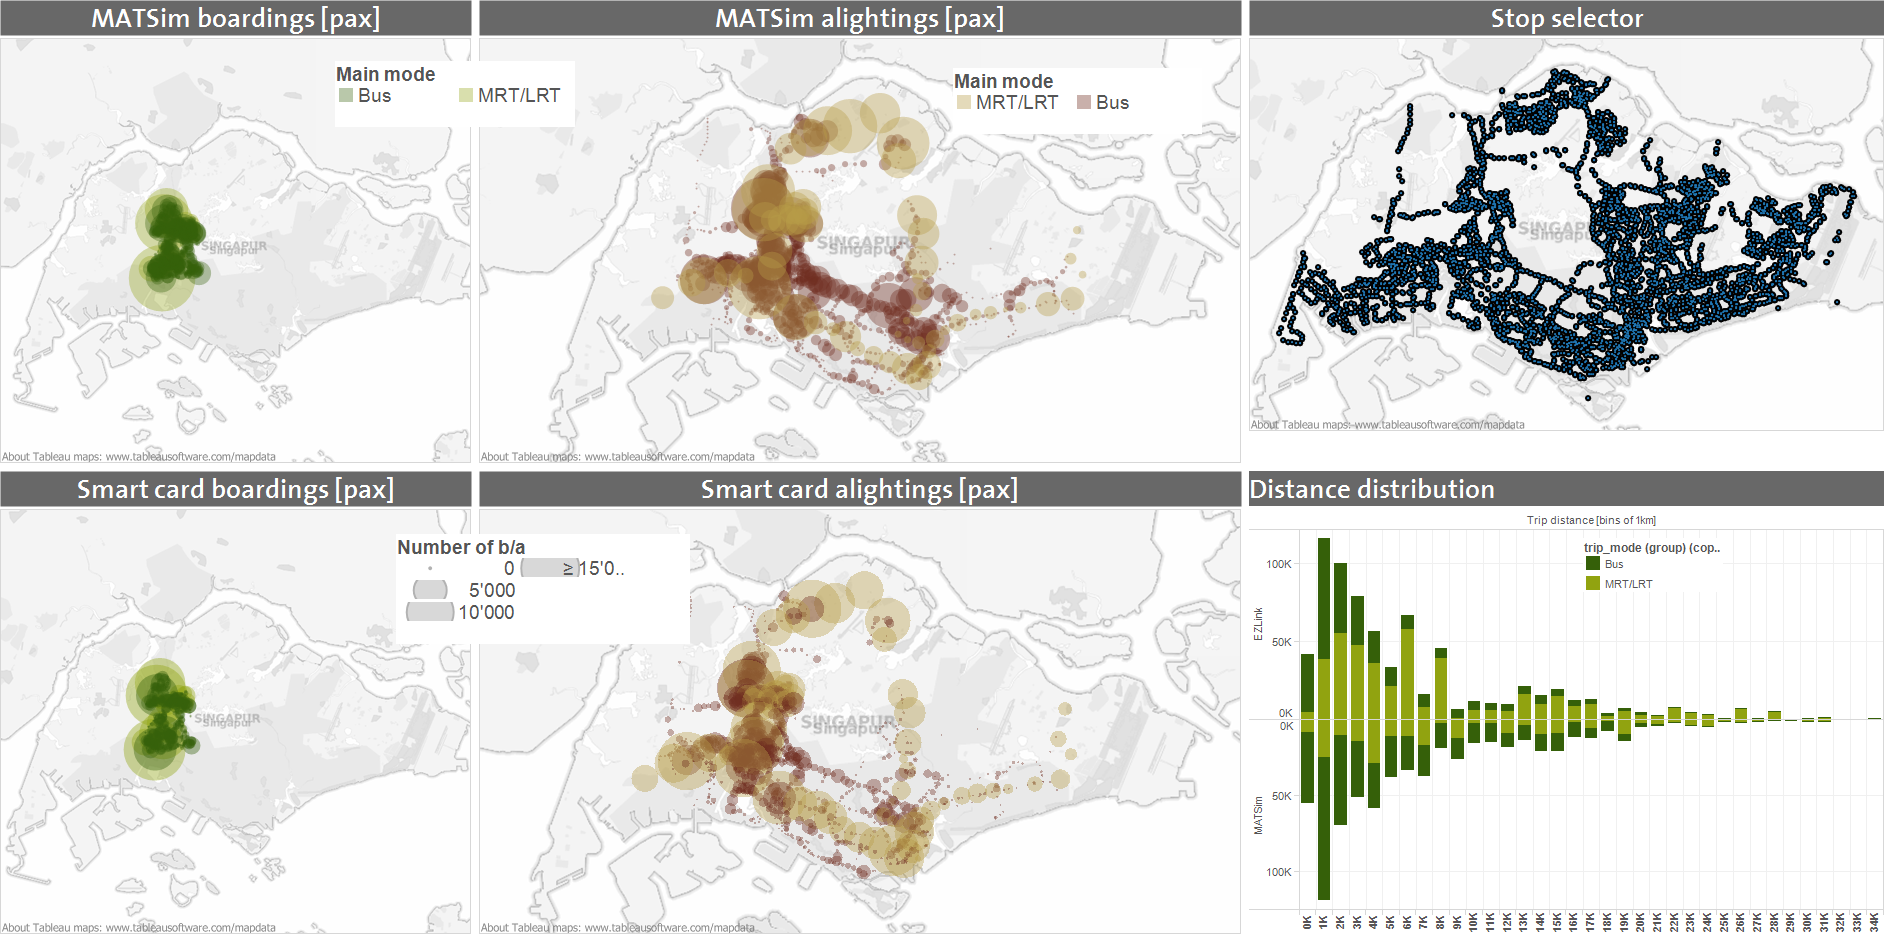
\includegraphics[width=0.4\textwidth, angle=0]{extending/figures/businessanalytics/tableau.png} \end{center}

This chapter is largely based on work in \citet[][]{ErathEtAl_EASTS_2013} where the interested reader will find references to further reading.
\section{Introduction}
\label{sec:analyticsIntro}
\paragraph{Agent-based simulation means lots of data}
Agent-based transport demand models require managing and integrating data sources that are several orders of magnitude larger than traditional aggregate models. In a truly disaggregate demand description, as can be found in our implementation of MATSim for Singapore, spatial data is at the level of individual buildings and land parcels, not zones; and travel demand takes the form of a full activity diary with connecting trips for every individual, based on their personal demographic attributes, instead of an aggregate number of trips from zone to zone for a time period under study. For this reason, the input data for an aggregate four-step (or related) demand model can generally be edited on a laptop using standard spreadsheet software, whereas agent-based modeling requires the manipulation and synthesis of large stores of structured, hierarchical data, frequently exceeding the capacity of most personal computers.

\paragraph{How MATSim stores data}
MATSim stores and retrieves data from XML, because XML can reflect the hierarchical structure of objects in the simulation, and is human-readable. But performing general exploratory analysis of large stores of XML data is usually poorly supported by most data analysis software packages, especially GIS-based systems. In order to perform analyses, expert knowledge of XML querying technologies like XPath and XQuery is required (or Java if one is to perform more specialized analysis on the objects themselves).  It is our experience that this specialized knowledge is lacking in transport and urban spatial planning practice. Therefore, in most applications of MATSim so far, authorities and other interested parties have to formulate their desired analysis in advance and have expert consultancies perform the analysis. Any queries resulting from the analysis means another cycle of consultation, and the value proposition to the client shrinks due to a lack of interactivity and feeling of ownership of the model. From our experience, this lack of a widely supported exploratory data analysis interface and the customer experience it creates, presents a considerable barrier to entry for many authorities and operators that are otherwise interested in using MATSim.

\paragraph{How customers interact with data: relational databases, GUI-driven interaction}
Most customers in the field of transport and urban spatial planning rely on mature, GUI-driven software such as ArcGIS \citep{ARC_GIS_2011}, EMME/3 \citep{EMME_Webpage_2015}, the PTV \citep{PTV_Webpage_2009} transport planning suite, even Microsoft Excel; all of which are capable of connecting to relational databases to perform queries on large datasets. Many analysts are capable of querying databases explicitly using the Structured Query Language (SQL), and the Open Database Connectivity (ODBC) standard allows software to connect to any relational database while being agnostic of the actual technology driving it. Importantly, many interactive exploratory data analysis software suites such as Tableau, Tibco Spotfire,  SAS and the open source R project support relational databases and ODBC.

\section{Requirements of a decision support interface to MATSim}
\label{sec:analyticsRequirements}
The event stream produced by the MATSim mobility simulation is a representation of what happened in the transport simulation at the atomic level. It could be fed into a relational database and an analyst knowledgeable in procedural languages could process it in arbitrary ways. But we foresee that there are general use case scenarios where most analysts will perform general tasks that can be standardized. To this end, we set about compiling a requirements specification of possible audiences and their use case scenarios, to come up with a general framework for interactive analysis and decision support that will satisfy most requirements. We developed a set of Java classes to process MATSim input and output in order to produce the tables in a relational database, according to an entity relationship diagram that should be intuitive and useful to a large user audience.

\subsection{Users}
The decision support tool presented in this chapter is geared to decision makers and researchers
in the fields of transport planning and operations, spatial planning and spatial economics and
geography. Generally speaking, it should serve professionals who are interested in mobility
and spatial analysis and understand the principles of transport modelling but do not have the
expertise to operate an agent-based transport simulation directly. Currently, we envision the
following stakeholders and some example questions for a decision-support system --- a non-exhaustive list that, we expect, will grow with time:
\paragraph{Transport planners}
How many trips occur where, when and what is the activity purpose?
What are the socio-demographic characteristics of the these persons?
\paragraph{Urban planners}
What are the temporal usage patterns of buildings and the surrounding neighbour-
hood?
What is the flow from public transport stops to surrounding buildings?
\paragraph{Policy-makers}
What are the costs and benefits of a new public transport service?
Who are the winners and losers from constructing a new road?
\paragraph{Public transport operators}
What is the breakdown of the ridership of certain bus lines?
\paragraph{Service industry}
Which customers are in catchment areas, separated by mode?

\subsection{Functional requirements}

The decision support framework should facilitate classic transport
appraisal methods such as cost/benefit analysis and evaluation of the spatial impact of transport
infrastructure and policy measures. The framework should allow any sort of spatial analysis on the finest level of granularity
provided by the transport model; usually individual buildings or parcels as well as public
transport stops and selected links such as count stations or tolled road segments. However, these geographic features should be indexed against transport zones or other geographic areas of interest to allow aggregation of results.
Furthermore, it should capture all temporal aspects of the simulation, as full temporal dynamics is a strong feature of the agent-based approach.

\section{General framework for decision support}
Figure~\ref{fig:analyticsFramework} shows the general framework as we envision it: data from various sources feed into a spatially-enabled database, with all geodata transformed to use the same spatial reference system (probably the same projection used for MATSim coordinates, allowing for simple distance calculations). Simple Java programs using the MATSim API and JDBC (Java Database Connectivity standard) produce XML input data for MATSim scenarios, and events from these scenarios are fed back into the database for comparison and validation. Analysts query the database to produce 'data cubes', which are aggregations and queries across many tables in the database designed for specific purposes, such as calibration and validation, location analysis, winner/loser analysis or other application-specific purposes.

\subsection{Entity relationship diagram (ERD) for general purpose analysis}

In terms of entity relationships, we decided that a travel diary format is especially suitable for comparison against other data sources for validation. Most travel surveys take the form of a diary recording travel time, purpose, mode; as well as aspects of the journey such as number of stages, transfer walking and waiting time, and in-vehicle time. Routines can be developed to transform survey data  and public transport smart card records into the same format with consistent coding. Figure~\ref{fig:analyticsERD} shows the entity relationship diagram  we propose, along with the primary/foreign key relationships between tables that facilitate aggregation and joining of e.g. personal/household attributes such as income with travel time experienced in the simulation.

\subsection{Interactive analysis using business analytics software}
Modern business analytics software such as Tableau \citep{Tableau_Webpage_2013} provide interactive aggregation and graphing of data from relational databases. While basic analysis of individual tables in our proposed ERD could already provide valuable insight to MATSim simulations, much richer analysis is possible when the relationships betweendifferent tables in the database are Graphical query building software can be used to construct SQL scripts of data cube requiring very little or no knowledge of SQL by the analyst. these cubes are fed into Tableau, which is designed with a relatively technology-agnostic audience in mind. Relying on the familiar paradigm of drag-and-drop interaction in a simple, well-documented GUI, the user constructs 'dashboards' summarizing information and allowing interactive aggregation or drilling-down across multiple dimensions.

Figure~\ref{fig:analyticsTableau} shows such a Tableau visualization comparing public transport ridership from a MATSim simulation against actual smart card data records (transformed into the travel diary format specified in the ERD). Figure~\ref{fig:analyticsJoin} shows the SQL query used to produce the data frame driving the Tableau analysis. The query exploits the primary/foreign key relationships in the database to perform rapid joins between the different tables.


% ------------
\createfigure%
{General framework of the decision support system}%
{General framework of the decision support system}%
{\label{fig:analyticsFramework}}%
{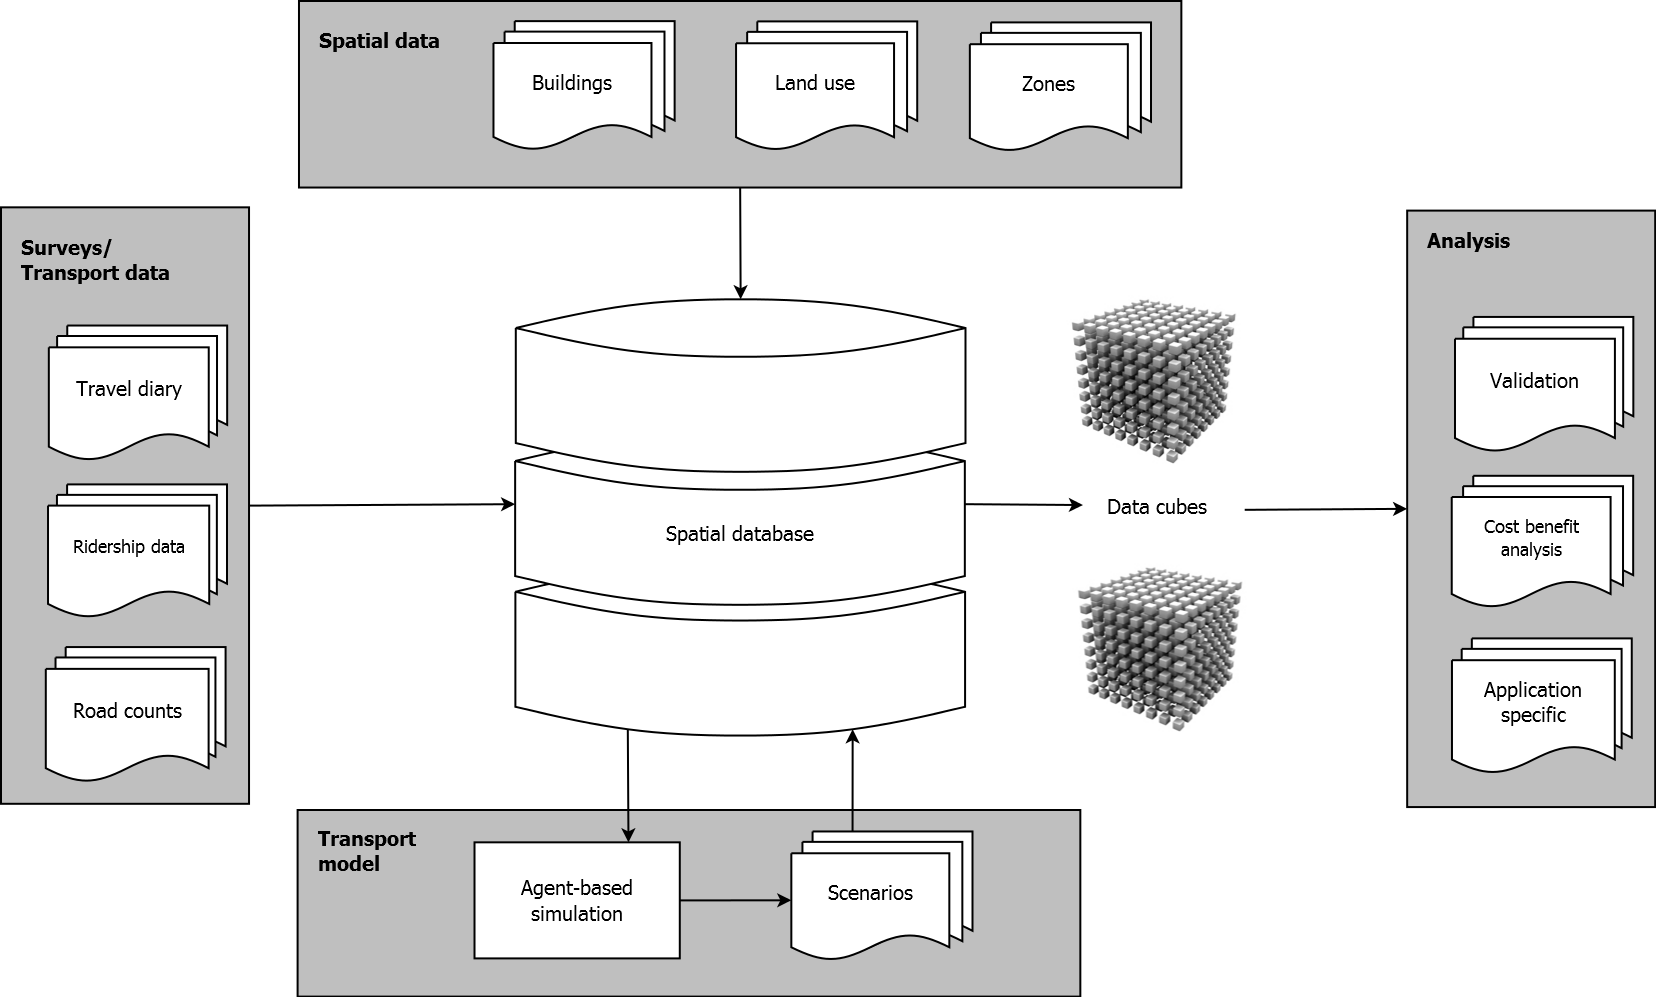
\includegraphics[width=0.65\textwidth, angle=0]{extending/figures/businessanalytics/general}}%
{}
% ------------

% ------------
\createfigure%
{Simplified entity relationship diagram showing shared keys across tables}%
{Simplified entity relationship diagram showing shared keys across tables}%
{\label{fig:analyticsERD}}%
{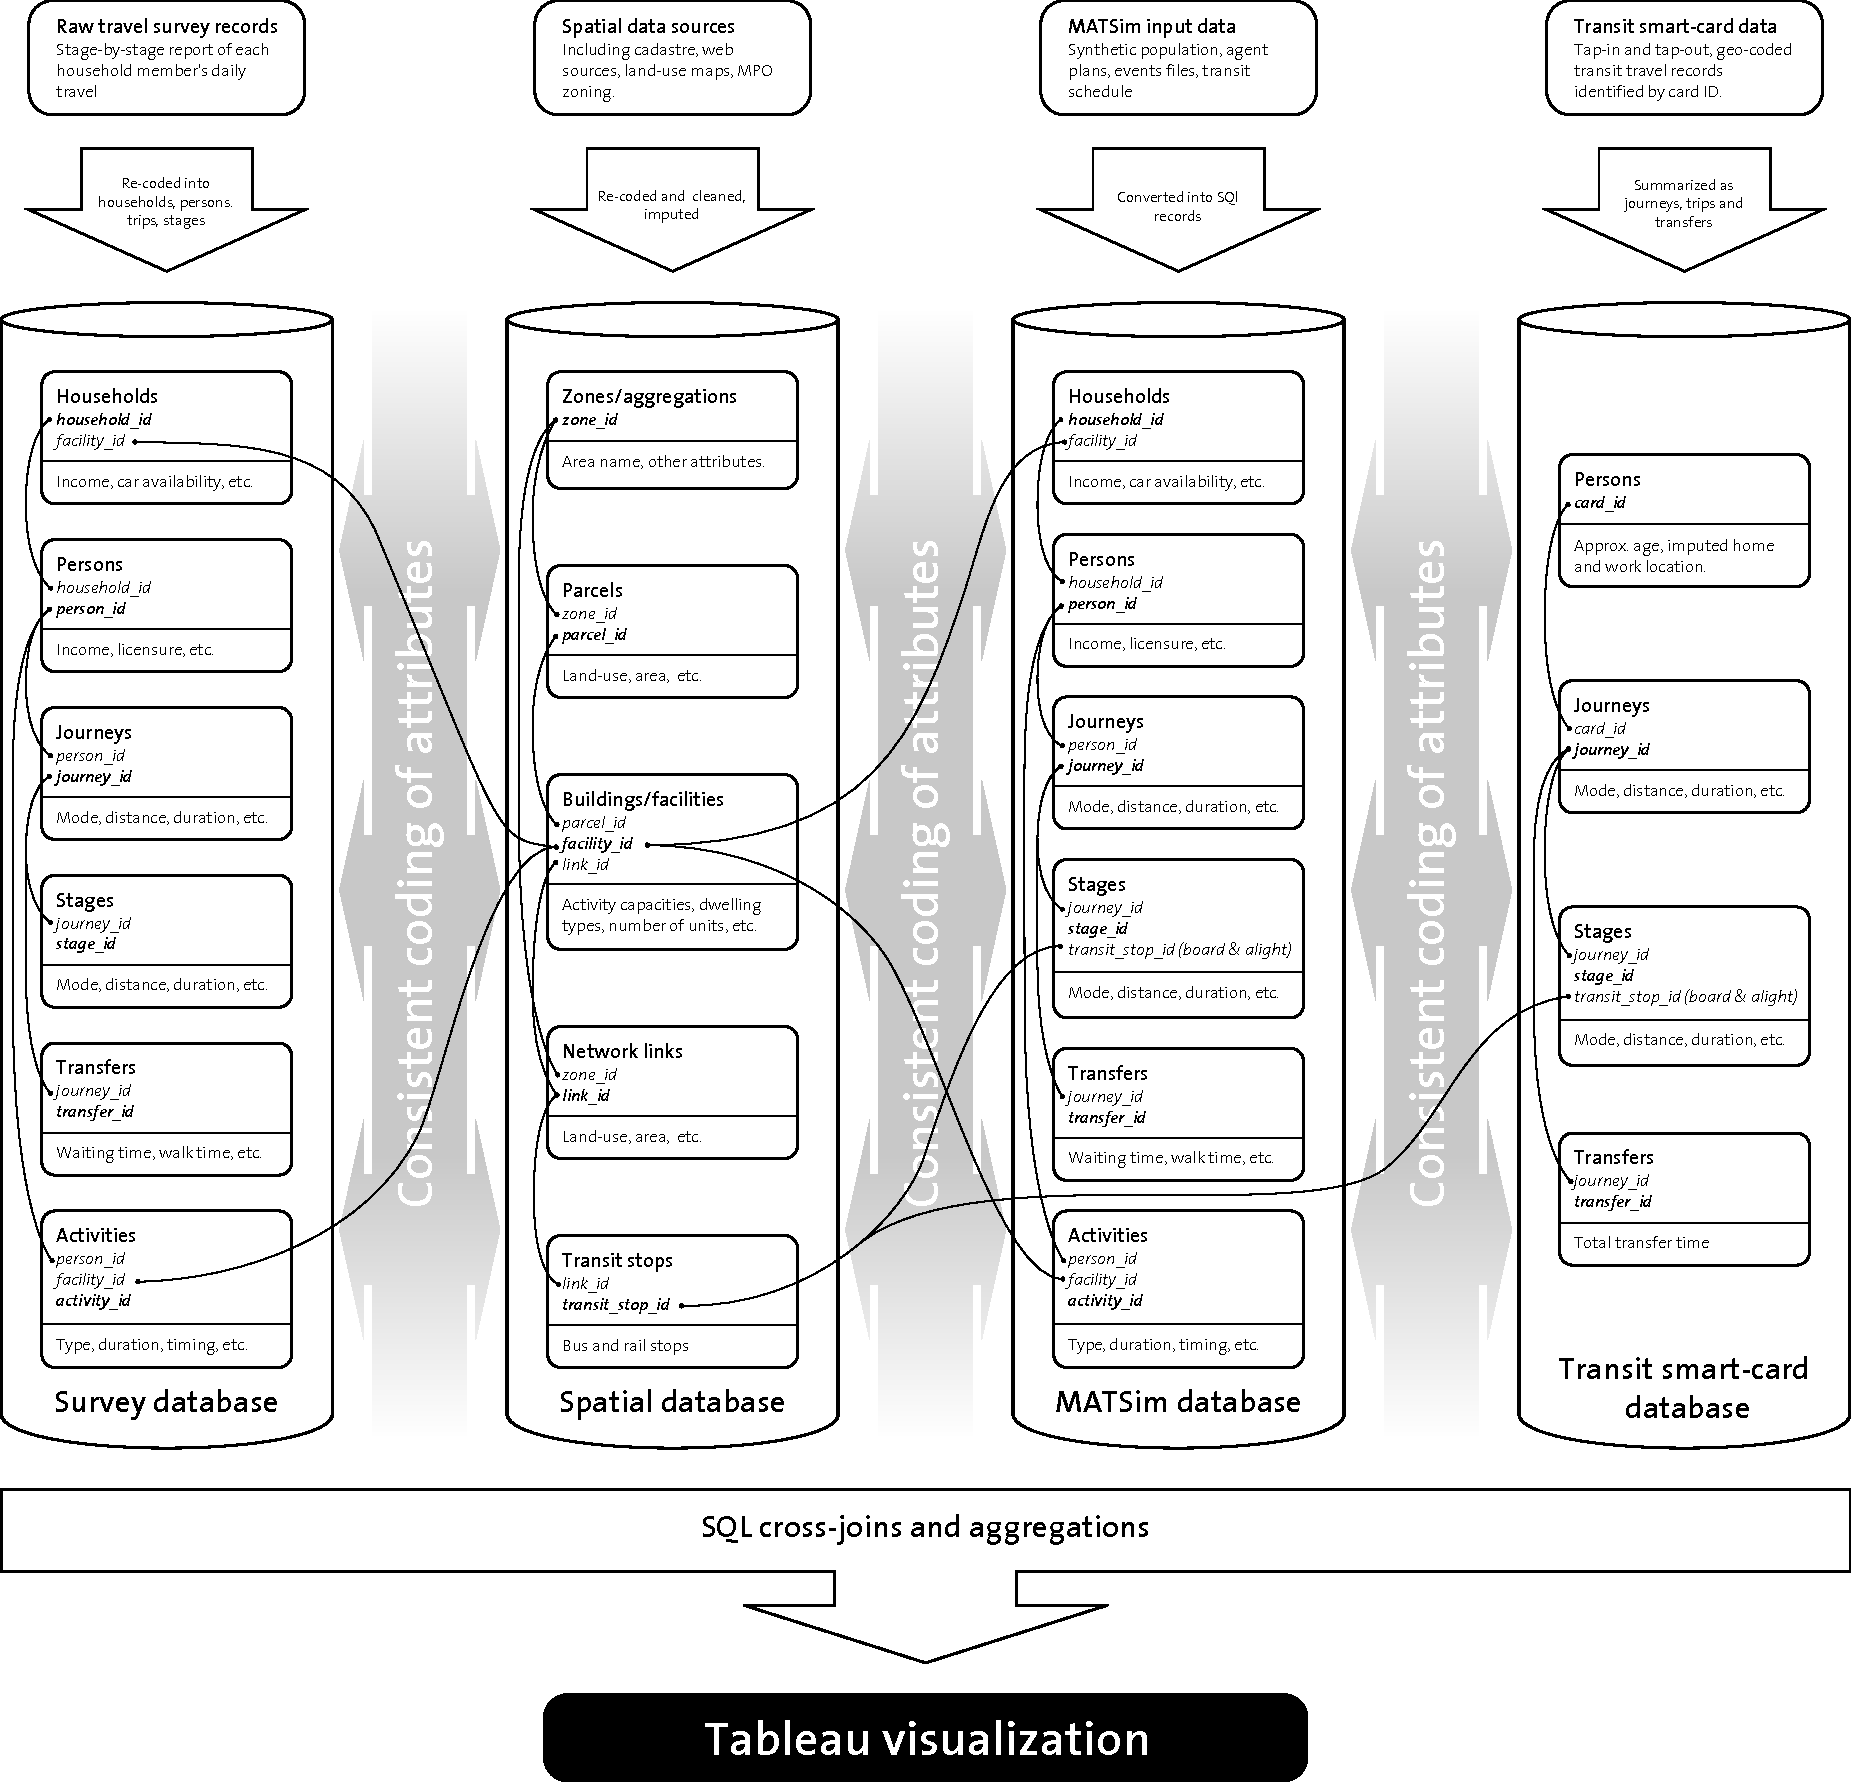
\includegraphics[width=0.65\textwidth, angle=0]{extending/figures/businessanalytics/schema}}%
{}
% ------------

% ------------
\createfigure%
{Tableau visualization}%
{Tableau visualization of public transport ridership from a MATSim simulation compared against actual smart card data records in Singapore}%
{\label{fig:analyticsTableau}}%
{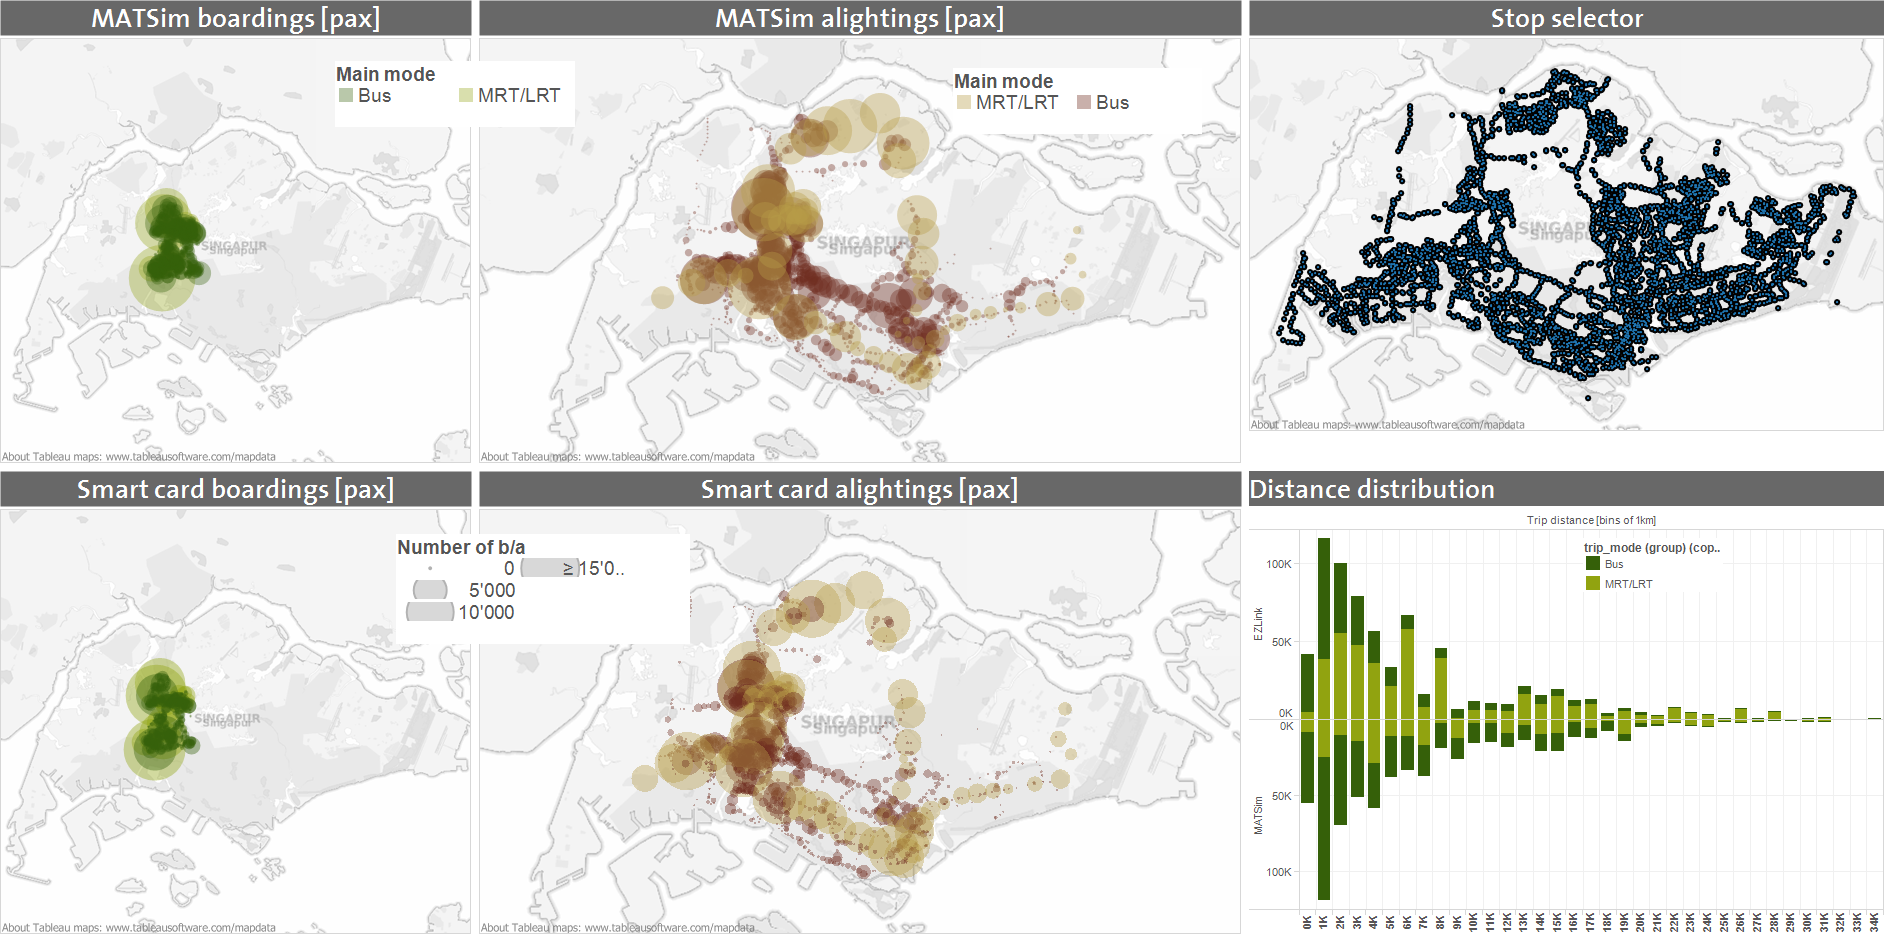
\includegraphics[width=0.25\textwidth, angle=0]{extending/figures/businessanalytics/tableau.png}}%
{}
% ------------

% ------------
\createfigure%
{Table joined in analytics software}%
{A diagram showing how the tables from Figure \ref{fig:analyticsERD} are joined together for visualization in business analytics software, e.g. Tableau, as shown in Figure~\ref{fig:analyticsTableau}}%
{\label{fig:analyticsJoin}}%
{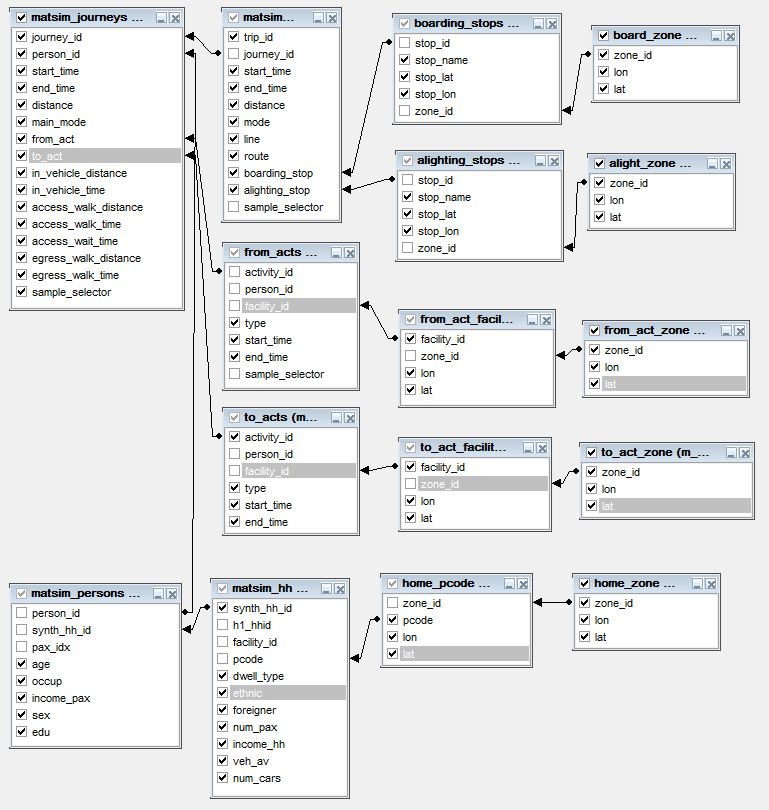
\includegraphics[width=0.65\textwidth, angle=0]{extending/figures/businessanalytics/join}}%
{}
% ------------



% ################################################################################################################
\section{Diaries from Events}
In the package \lstinline|playground.singapore.travelsummary| the reader may find a set of classes that will transform their MATSim simulation results into a set of travel diary tables, such as those discussed in the preceding section. The package contains a simple GUI class that can be run to specify input data XML files, the location to save output comma separated value (CSV) files, and other information such as a subscript appended to the end of file names to identify different scenarios. These CSV files can be read into a relational database of choice, or directly queried in Tableau or other interactive analysis software.

% ################################################################################################################




